\documentclass[12pt]{article}
\usepackage{amsmath}
\usepackage{tikz}
\usepackage{graphicx}
\newcommand{\ihat}{\boldsymbol{\hat{\textbf{$\imath$}}}}
\newcommand{\jhat}{\boldsymbol{\hat{\textbf{$\jmath$}}}}
\newcommand{\khat}{\boldsymbol{\hat{\textbf{k}}}}

\graphicspath{ {./images/} }
\begin{document}
\title{Statics Review}
\author{Aditya Dangra}
\date{\today}
\maketitle

\pagenumbering{roman}
\tableofcontents
\pagebreak
\pagenumbering{arabic}

\section{Chapter 1: General Principles}
Statics deals with the equilibrium of bodies, that is, those that are at rest or moving with constant velocity.
Its importance to the real world stems from the need to keep things from moving, such as buildings or bridges.

\subsection{Important Points}
The following points outline the foundations upon which the study of Statics is built upon.

\begin{itemize}
    \item Statics is the study of bodies that are at rest or moving with constant velocity \cite{hibbeler}.
    \item Newton's three laws of motion are integral to the study of statics and should be memorized.
    \item If size is negligible, then a system can be reduced to a single particle containing all of its mass.
    \item Concentrated forces are assumed to act at a single point on a body (In reality, all forces are distributed loads).
    \item The meter, second, and kilogram are base units of the SI system.
    \item The foot, second, and pound are base units of the Imperial system.
    \item Mass measures the quantity of matter that does not change depending on location. Weight refers to the gravitational attraction of the earth on a quantity of mass.
\end{itemize}

\subsection{General Procedure}
Attending lectures, reading books, and studying example problems help, but \textbf{the most effective way of learning is to \textit{solve problems}} \cite{hibbeler}.
The following is a generalized procedure that should apply to all problems and ensure success:

\begin{itemize}
    \item Read the problem and try to correlate the situation with the theory studied.
    \item Draw a free body diagram of the situation with all necessary forces, moments, and dimensions.
    \item Write out any relevant equations and diagrams.
    \item Solve the necessary equations in an efficient manner.
    \item Study the answer with technical judgement and common sense to determine whether it seems reasonable.
\end{itemize}

\subsection{Relevant Problems}
In Chapter 1, the problems focus on unit conversions and Newton's Law of Gravitation.
Some relevant problems include:

\begin{itemize}
    \item Unit Conversions:
    \begin{itemize}
        \item 1-2, 1-7, 1-9, 1-10, 1-14
    \end{itemize}
    \item Density and Gravitation:
    \begin{itemize}
        \item 1-17, 1-19, 1-21
    \end{itemize}
\end{itemize}

\pagebreak
\section{Chapter 2: Force Vectors}
A \textbf{scalar} is any positive or negative quantity that can be specified by its \textit{magnitude}.
A \textbf{vector} is any quantity that requires both a \textit{magnitude} and a \textit{direction} \cite{buckham}.
A vector is shown graphically by an arrow indicating the sense of direction and an angle $\theta$ between the vector and a fixed axis.

\subsection{Vector Operations}
Like scalars, vectors can also be added and multiplied, but a slightly different set of rules apply.

\subsubsection*{Multiplication by a Scalar}
When a vector is multiplied by a scalar, its magnitude will be increased by that amount. 
Multiplying by a negative reverses the direction of the vector.

\subsubsection*{Vector Addition}
Adding vectors is done \textit{tip to tail}, as in the second vector's tail is moved to the tip of the first vector (Figure 1).
The vector between the first tail and the final tip is the \textbf{resultant}, another vector.
Vectors can also be added component-wise, where the $x$-component of the resultant is the sum of the $x$-components of the vectors being added and so on.

\begin{figure}
\centering
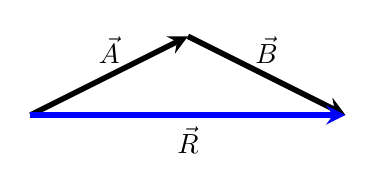
\begin{tikzpicture}
    \draw[line width=2pt, black, -stealth](0, 0) -- (2, 1) node[midway, above]{$\vec{A}$};
    \draw[line width=2pt, black, -stealth](2, 1) -- (4, 0) node[midway, above]{$\vec{B}$};
    \draw[line width=2pt, blue, -stealth](0, 0) -- (4, 0) node[midway, below, text=black]{$\vec{R}$};
\end{tikzpicture}
\caption{Adding two vectors \textit{tip to tail}}
\end{figure}

\subsubsection*{Vector Subtraction}
Vector subtraction is defined as a special case of vector addition.
Instead of being subtracted, the vector is multiplied by $-1$ and instead added (shown below).

\begin{equation*}
    \vec{R} = \vec{A} - \vec{B} = \vec{A} + \left(-\vec{B}\right)
\end{equation*}

\subsection{Force Components}
Forces can be represented with magnitude and direction but it is usually easier to work with components in the $x$, $y$, and $z$ directions.
It is possible to calculate the components using an angle and magnitude or with the \textbf{coordinate direction angles} $\alpha$ (alpha), $\beta$ (beta), and $\gamma$ (gamma).
Coordinate direction angles are measured between the vector and the \textit{positive} $x$, $y$, and $z$ axes.
$\alpha$, $\beta$, and $\gamma$ for a vector $\vec{A}$ are defined as:

\begin{align*}
    \cos{\alpha} &= \frac{A_x}{A} & \cos{\beta} &= \frac{A_y}{A} & \cos{\gamma} &= \frac{A_z}{A} \\
\end{align*}
The following identity also holds:
\begin{equation*}
    \cos^2{\alpha} + \cos^2{\beta} + cos^2{\gamma} = 1
\end{equation*}

Sometimes, the direction of a vector can be specified in terms of a \textbf{transverse angle} $\theta$ and an \textbf{azimuth angle} $\phi$, as shown in figure 2.
The formula to find the components should not be memorized, instead determined by trigonometry.

\begin{figure}[h]
\centering
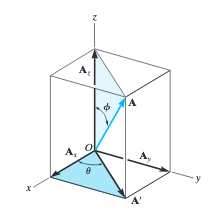
\includegraphics[scale=0.7]{transverse_azmuth.png}
\caption{A vector's direction in terms of $\theta$ and $\phi$ \cite{hibbeler}}
\end{figure}
\pagebreak

\subsection{The Dot Product}
The dot product can be used to find the angle between 2 vectors.
Expressed in equation form:
\begin{align*}
    \vec{A}\cdot\vec{B} &= AB\cos{\theta}\\
                        &= A_xB_x + A_yB_y + A_zB_z
\end{align*}
The magnitude of the projection of $\vec{A}$ onto $\vec{u_a}$ is determined from the dot product, $A_a = \vec{A}\cdot\vec{u}_a$.

\subsection{Relevant Problems}
In Chapter 2, the problems focus on working with Force Vectors, determining components from angles, and using the dot product.
Some relevant problems include:
\begin{itemize}
    \item Force Vectors:
    \begin{itemize}
        \item 2-2, 2-6, 2-7, 2-17, 2-19, 2-31, 2-43, 2-55
    \end{itemize}
    \item Cartesian Vectors:
    \begin{itemize}
        \item 2-61, 2-66, 2-70, 2-78, 2-86, 2-99, 2-103
    \end{itemize}
    \item The Dot Product:
    \begin{itemize}
        \item 2-106, 2-110, 2-113, 2-115, 2-130, 2-137
    \end{itemize}
\end{itemize}
\pagebreak

\section{Chapter 3: Particle Equilibrium}
\paragraph{}
When a body's forces' lines of action pass through a single point, the body can be thought of as a particle. 
For this particle to be in equilibrium, the net force must equal 0 ($\sum{\vec{F}} = 0$).

\paragraph{}
Accounting for all of the forces can be done with the help of a free-body diagram.
This diagram cuts the particle away from its surroundings and shows all forces acting on the particle with their known/unknown magnitudes and directions \cite{buckham}.

\paragraph{}
If the geometry is hard to visualize, it is easier to solve the system's equilibrium equations in the $x$, $y$, and $z$ directions.
\begin{align*}
    \sum{F_x} &= 0 & \sum{F_y} &= 0 & \sum{F_z} &= 0
\end{align*}

\subsection{Relevant Problems}
In Chapter 3, the problems focus on two-dimensional and three-dimensional particle equilibrium.
Some relevant problems include:
\begin{itemize}
    \item Two-dimensions:
    \begin{itemize}
        \item 3-7, 3-9, 3-23, 3-30, 3-31, 3-37, 3-42
    \end{itemize}
    \item Three-dimensions:
    \begin{itemize}
        \item 3-46, 3-47, 3-60, 3-67
    \end{itemize}
\end{itemize}

\section{Chapter 4: Force System Resultants}
Forces, along with a tendency to cause translation, also produce a tendency to cause rotation.
This effect is called a \textbf{moment} whose magnitude is the product of the magnitude of $\vec{F}$ and $d$, the perpendicular distance to the line of action of $\vec{F}$.

\subsection{The Cross Product}
\paragraph{}
Moments are three-dimensional vectors perpendicular to the plane containing the other two vectors.
The operation to describe this, the cross product, is not yet in our vector algebra toolkit, so we define the cross product of vectors $\vec{A}$ and $\vec{B}$ as a vector $\vec{C}$ with magnitude $C = AB\sin{\theta}$ and a direction as specified by the right-hand rule.

\paragraph{}
As with other vector operations, it is usually easier to work in terms of components, so the cross product can be written as:
\begin{equation*}
    \vec{A} \times \vec{B} = 
    \begin{vmatrix}
        \ihat  & \jhat  & \khat \\
        A_x    & A_y    & A_z \\
        B_x    & B_y    & B_z
    \end{vmatrix}
\end{equation*}

\subsection{Moments}
\paragraph{}
If a force $\vec{F}$ is $\vec{r}$ away from point $O$, the moment about point $O$ can be expressed using the cross product:
\begin{equation}
    \vec{M}_O = \vec{r} \times \vec{F}
\end{equation}

\paragraph{}
Since $\vec{F}$ is a sliding vector, we can make use of its \textit{principle of transmissibility}.
This principle states that any position vector $\vec{r}$ from point $O$ creates \textit{the same moment} about point $O$, as shown in figure 3.

\begin{figure}[h]
\centering
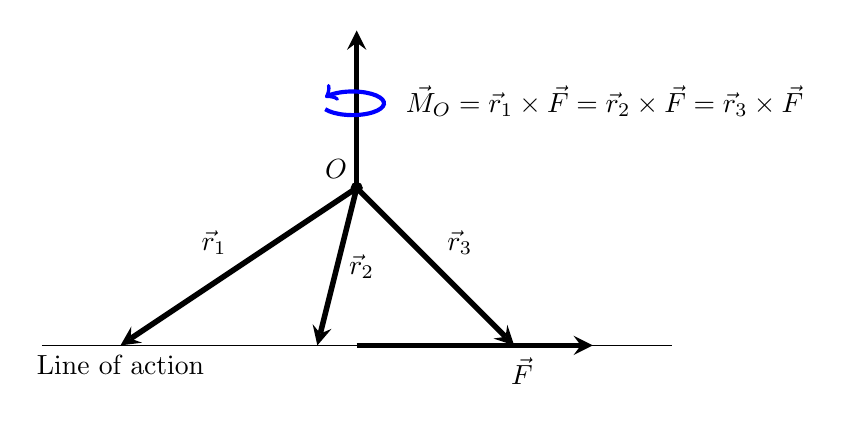
\begin{tikzpicture}
    \draw[fill] (0, 2) circle [radius=0.07];
    \draw (-4, 0) -- (4, 0);
    \draw[line width=2pt, -stealth] (0, 2) -- (0, 4);
    \draw[line width=2pt, -stealth] (0, 2) -- (-3, 0) node[midway, above left] {$\vec{r}_1$};
    \draw[line width=2pt, -stealth] (0, 2) -- (-0.5, 0) node[midway, right] {$\vec{r}_2$};
    \draw[line width=2pt, -stealth] (0, 2) -- (2, 0) node[midway, above right] {$\vec{r}_3$};
    \draw[line width=2pt, -stealth] (0, 0) -- (3, 0) node[pos=0.7, below] {$\vec{F}$};
    \draw[x=0.40cm, y=0.15cm, blue, line width=1.5pt, -stealth, ->] (-1, 20) arc(-150: 150: 1 and 1);

    \node[above left] at (0, 2) {$O$};
    \node[right] at (0.5, 3.1) {$\vec{M}_O = \vec{r}_1 \times \vec{F} = \vec{r}_2 \times \vec{F} = \vec{r}_3 \times \vec{F}$};
    \node[below] at (-3, 0) {Line of action};
\end{tikzpicture}
\caption{The principle of transmissibility.}
\end{figure}


\pagebreak
\addcontentsline{toc}{section}{References}
\begin{thebibliography}{2}
    \bibitem{hibbeler}
    R. C. Hibbeler, \textit{Engineering Mechanics: Statics \& Dynamics (Fourteenth Edition)}, Pearson Prentice Hall, Hoboken, New Jersey, 2016.
    \bibitem{buckham}
    B. Buckham, \textit{ENGR 141 Lecture}, University of Victoria, Victoria, B.C., 2019.
\end{thebibliography}

\end{document}